\documentclass[11pt, fleqn]{article}

\usepackage{amsmath}
\usepackage{amsfonts}
\usepackage{amsthm}
\usepackage[margin=1in]{geometry} % To set the margin widths
\usepackage{graphicx}
%\usepackage{hyperref}
\usepackage{listings}
\usepackage{multirow}
\usepackage{tabularx}
\usepackage{varioref}
\usepackage{cleveref}  % this redefines vref to use cleverref
\usepackage{siunitx}
%\usepackage{subcaption}
\usepackage{subfig}
\usepackage{titlesec}
\usepackage{bm}

\crefname{equation}{equation}{equations}
\crefname{figure}{figure}{figures}

\sisetup{output-exponent-marker=\textsc{e}}

\titleformat{\section}[block]{\bfseries}{\thesection}{1em}{}


\setlength{\parskip}{12pt} % Sets a blank line in between paragraphs
\setlength\parindent{0pt} % Sets the indent for each paragraph to zero

\begin{document}

\title{Big Data: Homework 7}
\author{Will Clark \& Matthew DeLio \\ 41201-01}
\date{\today}
\maketitle

\section{Foreign Exchange Factor Modeling} \label{sec:intro}

% From Wikipedia: Principal component analysis (PCA) is a statistical procedure that uses an orthogonal transformation to convert a set of observations of possibly correlated variables into a set of values of linearly uncorrelated variables called principal components. 

\section{Principal Components Analysis} \label{sec:pca}
% Fit, plot, and interpret principal components.

At first glance, our data set of monthly foreign exchange rates seems to have a lot of noise and very little signal. The goal of principal components analysis is to see if there are any patterns connecting variables in our data set, and if there are, use these relationships to reduce the dimensionality of our data. To this end, we use \texttt{prcomp} to find the principal components of foreign exchange movements. For each observation $i$, which is a month of foreign exchange rates for 23 currencies, the method estimates:
\begin{equation}
E[x_i] = \varphi_i v_{i,1} + \varphi_2 v_{i,2} + ... + \varphi_k v_{i,k}
\end{equation}
We can now represent the data along the new set of dimensions $v_{i,j}$, which should reveal any latent patterns that were not observable when we were looking at the set of original dimensions $x_{i,j}$.

We can start by looking at the scree plot of our PCA, shown in Figure~\ref{fig:screeplot}. This shows us the sorted eigenvalues of the covariance matrix of the scaled data; the highest eigenvalue is the principal component that explains most of the variation in the data. The steep drop off after the first bar tells us that the first principal component explains a large degree of the variability in our data.

\begin{figure}[!htb]
  \centering
  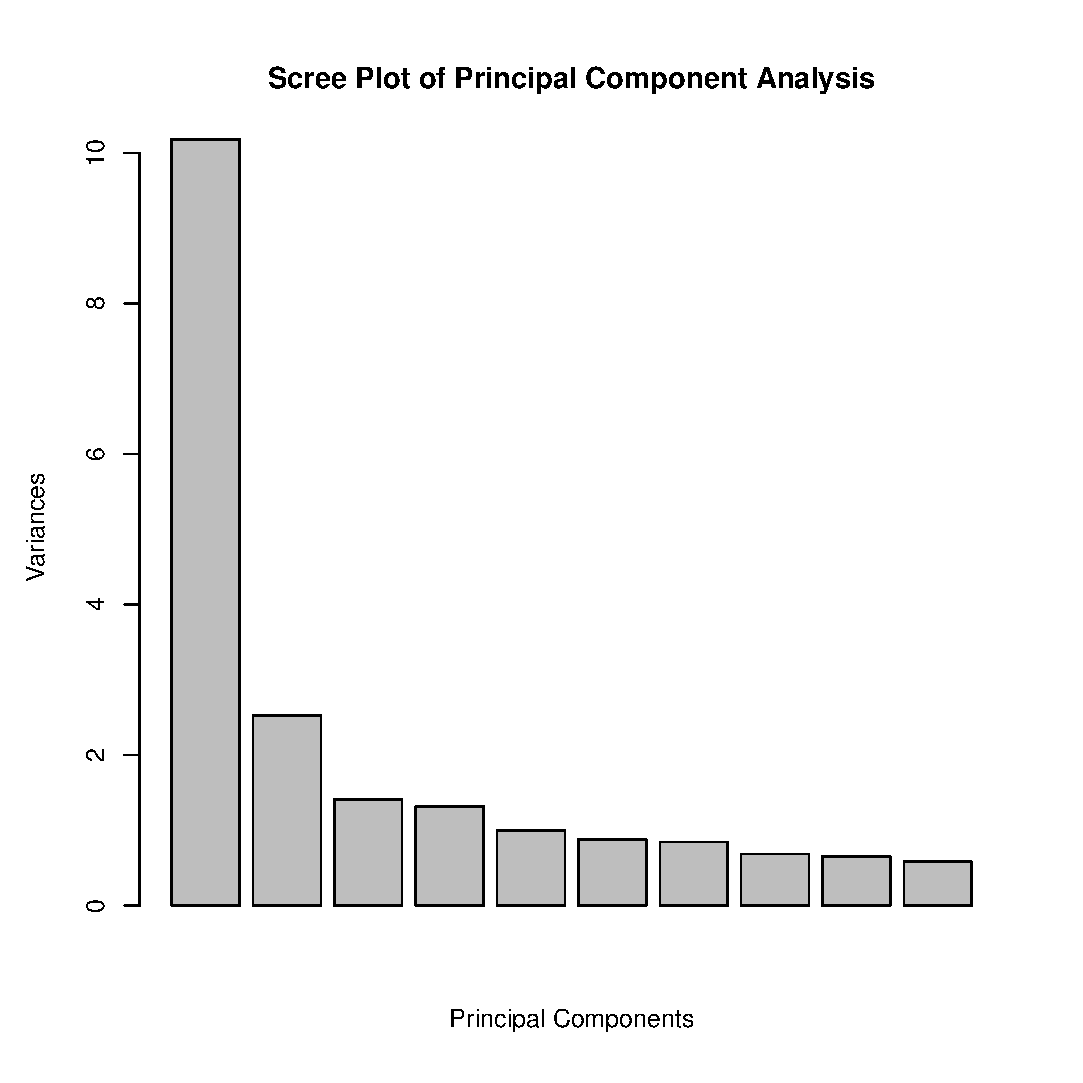
\includegraphics[scale=.5]{screeplot.eps}
  \caption{Foreign Exchange PCA Scree Plot}
  \label{fig:screeplot}
\end{figure} 

We can look at the rotations on the first principal component and see if there is any obvious interpretation. Figure~\ref{fig:pc1_pegs} shows the rotations of PC1 on each country; countries in red have floating exchange rates and countries in blue have fixed exchange rates (Venezuela, China, Hong Kong, and Sri Lanka). Given that all the pegged exchange rates are on one side and all the floating rates are on the other, we can tentatively conclude that the first principal component is really telling us about the fixed/floating divide. It makes sense that most of the variation in exchange rates would occur between those that are allowed to move freely and those that are not, and since PCA is supposed to find the latent sources of variation, it follows that this is the first dimension on which it chooses to sort the data.

\begin{figure}[!htb]
  \centering
  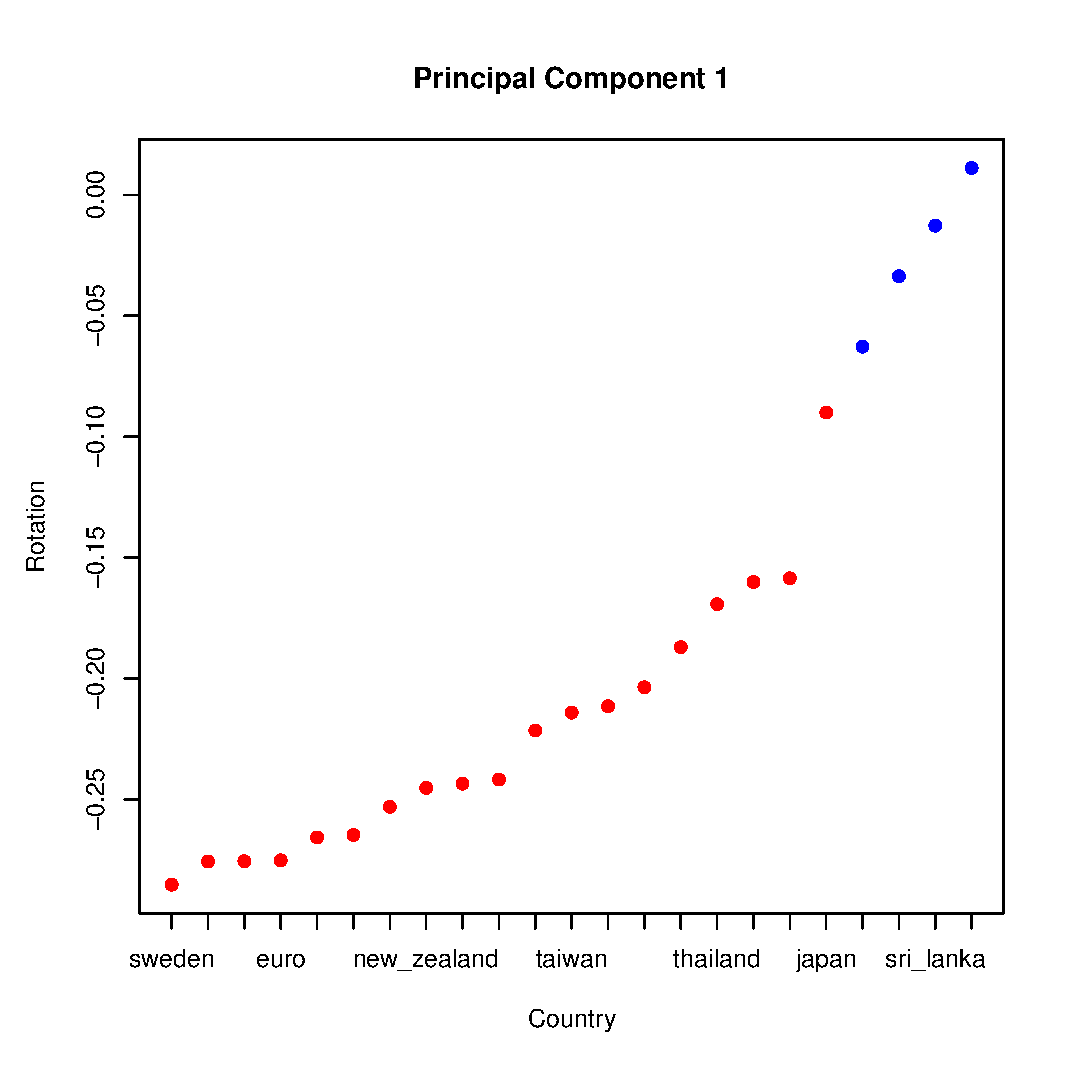
\includegraphics[scale=.5]{pc1_pegs.eps}
  \caption{Distribution of First Principal Component}
  \label{fig:pc1_pegs}
\end{figure} 

\section{S\&P 500 Returns on Currency Factors} \label{sec:sp500}
% Regress SP500 returns onto currency movement factors,
% using both ‘glm on first K’ and lasso techniques.
% Use the results to add to your factor interpretation.

We can use our principal components from Section~\ref{sec:pca} to estimate monthly returns of the S\&P 500. First, we use only the first principal component in a standard regression model:
\begin{equation}
R_{SP,i} = \alpha + \beta_1 z_{1,i} + \varepsilon_{i}
\end{equation}
where $z_{1,i}$ is each observation projected in $v_{i,j}$ space. The in-sample $R^2$ of this regression is around 16 percent. Instead of running a standard linear regression on only one component, we can throw all the principal components into a lasso and see which coefficients are chosen. The model selected by the various decision criteria are shown in Table~\ref{tab:spreg_ics}. The model chosen by CV.min includes 16 of the possible 23 covariates, which is a fairly complex model given that PCA is intended to be a dimension reduction exercise. 

% latex table generated in R 3.2.0 by xtable 1.7-4 package
% Thu May 28 23:07:58 2015
\begin{table}[ht]
\centering
\begin{tabular}{rrrr}
  \hline
 & $\log(\lambda)$ & $R^2$ & Covariates Selected \\ 
  \hline
AICc & -5.83 & 0.49 &  13 \\ 
  AIC & -6.20 & 0.52 &  16 \\ 
  BIC & -5.41 & 0.43 &  10 \\ 
  CV.Min & -6.20 & 0.37 &  16 \\ 
  CV.1se & -5.08 & 0.26 &   9 \\ 
   \hline
\end{tabular}
\caption{ICs for S\&P500 Returns Regressed on FX Principal Components} 
\label{tab:spreg_ics}
\end{table}


The average out-of-sample $R^2$ of the cross-validated lasso regressions are 31 percent (for the CV.min model) and 21 percent (for the CV.1se model), so adding the extra set of principal components does increase the predictive accuracy of the model relative to the simple linear regression on only one principal component. Interestingly, the principal component with the highest coefficient in the CV.min lasso regression is PC23, the one that explains the least variation in the data set. If we look at the rotations on PC23, we see that all 21 are basically equal to zero, and one is very high and one is very low. The two outliers are the Euro and the Danish krone, which is pegged to the Euro. This means that the strongest predictor of S\&P returns in the currency data is just the US/EUR exchange rate, even though this is the dimension that explains the least amount of variation in the data.

\section{Regression on All Covariates} \label{sec:regall}

\end{document}